%% TFScope — Nature Methods submission
%% Compile: pdflatex && bibtex && pdflatex && pdflatex

\documentclass[11pt,letterpaper]{article}

% ── packages ─────────────────────────────────────────────────────────────────
\usepackage[margin=1.0in]{geometry}
\usepackage{setspace}
\doublespacing
\usepackage{fontenc}
\usepackage[utf8]{inputenc}
\usepackage{microtype}
\usepackage{amsmath,amssymb}
\usepackage{graphicx}
\usepackage{xcolor}
\usepackage{booktabs}
\usepackage{array}
\usepackage{tabularx}
\usepackage{caption}
\usepackage{subcaption}
\usepackage[numbers,sort&compress]{natbib}
\usepackage{hyperref}
\hypersetup{colorlinks=true, linkcolor=blue!60!black, citecolor=blue!60!black, urlcolor=blue!60!black}
\usepackage{lineno}
\linenumbers

% ── formatting ───────────────────────────────────────────────────────────────
\captionsetup{labelfont=bf, font=small, width=\linewidth}
\renewcommand{\figurename}{Fig.}
\newcommand{\ie}{\textit{i.e.}}
\newcommand{\eg}{\textit{e.g.}}
\newcommand{\ts}{\textasciitilde}

% section headings use default article bold styling

% ── title block ──────────────────────────────────────────────────────────────
\title{\textbf{TFScope: Sequence-Only Prediction of Transcription Factor
DNA-Binding Specificity with a Contact-Aware Protein Language Model}}

\author{
  Lei Huang$^{1}$~[co-authors TBD]\\[6pt]
  \small $^1$Department of Pathology, Massachusetts General Hospital and
         Harvard Medical School, Boston, MA 02114, USA\\
  \small Correspondence: lhuang34@mgh.harvard.edu
}
\date{}

% ─────────────────────────────────────────────────────────────────────────────
\begin{document}
\maketitle

% ─────────────────────────────────────────────────────────────────────────────
\begin{abstract}
\noindent
The DNA-binding specificity of a transcription factor (TF), summarized as a
position weight matrix (PWM), is a foundational quantity in gene regulation, yet
most TFs across the proteome have never been experimentally characterized and the
leading computational predictors require an experimentally solved or modeled
protein--DNA complex at inference. Here we present \textbf{TFScope}, a framework
that predicts PWMs directly from TF amino-acid sequence, with no structural input.
TFScope couples a protein language model encoder (ESM-2, 650\,M parameters) with
low-rank adaptation, dual-stream gated pooling of the DNA-binding domain (DBD), a
family-conditioned mixture-of-experts decoder, and a contact-aware cross-attention
head that localizes specificity-determining residues. On the 130-TF blind split of
the structure-based state-of-the-art DeepPBS, TFScope exceeds it on 8 of 11
motif-level metrics (mean per-column Pearson $r$ 0.802 vs.\ 0.750); even with
retrieval disabled, the sequence encoder alone already matches DeepPBS (0.749).
Under a 40\%-identity out-of-distribution benchmark TFScope attains mean $r$=0.535,
and leave-family-out analysis exposes a \ts0.48 sequence-only transfer floor.
Cross-attention recovers the canonical zinc-finger and basic-helix--loop--helix
recognition codes from sequence alone, and identifies long C2H2 zinc-finger arrays
as the prediction frontier. TFScope enables proteome-scale specificity annotation
at negligible cost.
\end{abstract}

% ─────────────────────────────────────────────────────────────────────────────
\section*{Introduction}

The sequence preference of a transcription factor for its genomic binding sites is
one of the central determinants of where, when, and how strongly a gene is
expressed. Encoded in the physico-chemical interface between a TF's DNA-binding
domain and the DNA double helix~\cite{Stormo2000,Luscombe2001}, this preference is
conventionally summarized as a position weight matrix (PWM): a compact, additive
model of the per-position base frequencies in bound sites. PWMs underpin nearly
every downstream analysis of gene regulation, from scanning genomes for regulatory
elements and reconstructing gene regulatory networks, to interpreting the
functional consequences of non-coding genetic variation that disrupts or creates
binding sites~\cite{Deplancke2016,Zhou2017}. Because mutations that alter TF
binding contribute to developmental disorders and cancer, and because engineered
TFs are increasingly used as tools in synthetic biology, accurate, proteome-scale
knowledge of binding specificity has both basic and translational value.

Despite decades of effort, experimentally determined specificities remain sparse.
High-throughput assays such as protein-binding microarrays~\cite{Berger2006},
HT-SELEX~\cite{Jolma2013}, and ChIP-seq have characterized only a fraction of the
\ts1,600 human TFs~\cite{Lambert2018,Vaquerizas2009}, and coverage is far poorer
across the broader eukaryotic proteome and for the many allelic and paralogous
variants whose specificities differ subtly but consequentially. Each assay is
laborious, organism- and condition-specific, and cannot keep pace with the rate at
which new TF sequences are catalogued. A predictive model that maps amino-acid
sequence directly to binding specificity would therefore fill a persistent and
widening gap.

Computational approaches to this problem fall into two broad classes, each with a
characteristic limitation. The first encodes hand-derived ``recognition codes,''
most famously the Cys$_2$His$_2$ zinc-finger code in which a small set of
recognition-helix residues specify the contacted DNA
triplet~\cite{Pavletich1991,Wolfe2000}; such codes are accurate within the family
they were derived for but do not generalize across the full diversity of TF
structural classes. The second class learns directly from functional genomics
data~\cite{Alipanahi2015,Zhou2017}, but these models are trained per-TF or
per-cell-type and presuppose the very experimental data we lack for uncharacterized
factors. Most recently, structure-based deep learning has set the state of the art:
DeepPBS~\cite{Mitra2024} reads DNA base preferences directly from the heavy-atom
contact geometry of a docked protein--DNA complex and, combined with advances in
structure prediction~\cite{Jumper2021}, can in principle be applied proteome-wide.
In practice, however, the structure requirement is a fundamental bottleneck:
accurate docked complexes are unavailable for most TF--DNA systems, modeling each
complex is computationally expensive, and prediction quality degrades when the
input structure is itself a prediction rather than a crystal.

Protein language models (PLMs) offer a route around the structure bottleneck.
Trained on hundreds of millions of natural sequences, models such as
ESM-2~\cite{Lin2023} capture evolutionary, structural, and functional regularities
that transfer to diverse downstream tasks~\cite{Elnaggar2022}. Crucially, the
specificity of a TF is governed by a small number of base-contacting residues in
its DBD~\cite{Najafabadi2015,Wolfe2000}, and these residues leave detectable
imprints in co-evolutionary and language-model representations. We hypothesized
that a PLM encoder, fine-tuned on the DBD with low-rank
adaptation~\cite{Hu2022}, would expose enough of this signal to predict binding
specificity from sequence alone, without recourse to any three-dimensional
structure.

Here we introduce TFScope, a sequence-only framework for PWM prediction. TFScope
encodes the TF through a PLM backbone, pools DBD-focused and global
representations, decodes through a family-conditioned mixture-of-experts
layer~\cite{Dai2024}, and emits a gated PWM through a contact-aware cross-attention
head that learns to attend to specificity-determining residues. An optional
retrieval branch supplies nearest-neighbor PWMs from experimentally characterized
TFs, providing an explicit, learned analogue of the homology transfer long used
informally in structural bioinformatics. We benchmark TFScope against the
structure-based state of the art under three regimes of increasing stringency,
dissect its behavior on well-characterized factors to show that it recovers
canonical recognition codes from sequence alone, and delineate honestly where it
generalizes and where it does not.

% ─────────────────────────────────────────────────────────────────────────────
\section*{Results}

\subsection*{A sequence-only framework for binding-specificity prediction}

TFScope maps a TF amino-acid sequence to a $4 \times L$ PWM through five stages
(Fig.~\ref{fig:architecture}). The \textit{encoder} is ESM-2 (650\,M parameters,
frozen)~\cite{Lin2023} with LoRA adapters (rank 16, $\alpha$ 32) on its last six
transformer layers (\ts491\,K trainable parameters); a learned DBD indicator
embedding marks residues inside the annotated domain, biasing representation
toward the recognition interface. \textit{Dual-stream gated pooling} summarizes the
sequence with two attention-pooled vectors — one over the whole protein, one
restricted to the DBD — which are concatenated and projected to a 512-dimensional
joint representation. A \textit{family-conditioned mixture-of-experts (MoE)
decoder}~\cite{Dai2024} (12 routed plus 1 shared expert, top-2 routing) is
conditioned on semantic family embeddings derived from PLM encodings of
family-level descriptions, so that even a structurally unfamiliar TF receives a
meaningful prior without any label leakage. A \textit{contact-aware cross-attention
head} maps PWM-column queries onto DBD residues; a residual branch
($z = z_{\mathrm{prior}} + \lambda\,\Delta z_{\mathrm{contact}}$) with cosine
attention and row-diversity and hub penalties adds 0.55\,M trainable parameters
while leaving the rest of the model frozen. Finally, a \textit{position gate}
selects information-rich columns and a regression head emits per-column base
frequencies; an optional retrieval branch injects $K$=3 nearest-neighbor PWMs,
indexed with leave-gene-out (LGO) hygiene, before the decoder.

\subsection*{Sequence-only prediction rivals structure-based specificity models}

We compared TFScope with DeepPBS~\cite{Mitra2024} on the latter's 130-TF blind test
split, applying two evaluation protocols identically to both methods. The
\textit{oracle-aligned} protocol trims each prediction to the target's
information-rich core (per-position information content, IC\,$\geq$\,0.25) and
grants oracle offset and reverse-complement alignment, isolating base-composition
accuracy from placement error. The \textit{canonical-fixed} protocol independently
canonicalizes prediction and target and grants no alignment, reflecting deployment.

Under oracle alignment, TFScope exceeded DeepPBS on 8 of 11 metrics across the 116
TFs both methods cover (Table~\ref{tab:bench1}). Mean per-column Pearson $r$ rose
from 0.750 to \textbf{0.802}, median $r$ from 0.759 to \textbf{0.831}, top-1 base
accuracy from 0.793 to \textbf{0.836}, Matthews correlation from 0.698 to
\textbf{0.765}, and mean absolute error fell from 0.133 to \textbf{0.108}; DeepPBS
retained an edge only on the two calibration metrics (cross-entropy and KL
divergence). Disabling the contact-aware branch — leaving only the frozen prior
($-$contact) — dropped mean $r$ to 0.701, attributing a $+$0.10 gain to a branch
that adds just 0.55\,M parameters.

The structural and sequence views diverge sharply on individual factors. For the
three-zinc-finger protein Egr1 (Zif268; PDB 1a1g), whose 10-bp GC-rich site is read
finger-by-finger through recognition-helix residues at positions $-1$, $+3$, and
$+6$ of each finger~\cite{Pavletich1991,Wolfe2000}, TFScope reconstructed all three
GCG subsites from sequence alone (oracle $r$=0.990), whereas DeepPBS, operating on
the same crystal complex, recovered essentially only the first guanine
($r$=0.776; Fig.~\ref{fig:egr1}). That a sequence model recovers the canonical
zinc-finger code more faithfully than a structure model reads it from atoms
illustrates how much specificity information the PLM representation already
encodes.

These oracle-aligned figures are upper bounds. When the alignment oracle is removed,
both methods lose \ts0.43 in mean $r$ and converge to a statistical tie (TFScope
0.420, DeepPBS 0.419; Table~\ref{tab:bench1}). Registration — placing the motif in
the correct frame and strand — is thus the dominant residual error for every method
evaluated, structure-based included, and is the clearest target for future
architectural work rather than a deficiency specific to TFScope.

\subsection*{Retrieval augmentation emulates homology transfer}

A central question is whether TFScope's advantage rests entirely on its retrieval
branch. It does not. With retrieval disabled, the sequence encoder alone reached
mean $r$=0.749 on the 130-TF split — statistically indistinguishable from DeepPBS
(0.750) and already ahead of it on top-1 accuracy (0.797 vs.\ 0.793) and Matthews
correlation (0.699 vs.\ 0.698; Fig.~\ref{fig:rag}, Table~\ref{tab:rag}). In other
words, a model that has never seen a single atomic coordinate matches the
structure-based state of the art from sequence alone. Re-enabling retrieval then
extends this parity into a clear lead across all base-composition metrics, raising
mean $r$ to 0.802 ($+$0.053).

The retrieval branch behaves as a learned homology-transfer operator: when an
experimentally characterized relative of the query exists in the reference set, its
PWM supplies a strong prior that the decoder weighs against its own sequence-derived
estimate, much as a structural biologist would transfer specificity by homology.
This interpretation makes leakage hygiene essential — building the index without
leave-gene-out exclusion permits a TF to retrieve a same-gene donor and inflates
performance spuriously; all reported figures use the LGO index.

\subsection*{TFScope generalizes to sequence-distant transcription factors}

Because near-homologues of test TFs may appear in the DeepPBS training data, strong
performance on that split could reflect memorization as much as genuine
sequence-to-specificity learning. To test out-of-distribution generalization we
constructed \textit{cluster40}, partitioning 1,320 unique proteins into 389 clusters
by CD-HIT~\cite{LiGodzik2006} at 40\% identity and splitting them, family-stratified,
into 2,983 training, 625 validation, and 639 test PWMs such that no test TF shares
$>$40\% identity with any training TF.

Trained from scratch on this split, TFScope reached mean oracle $r$=\textbf{0.535}
(median 0.505) on the held-out set (Fig.~\ref{fig:ood};
Table~\ref{tab:ood}), with consistent supporting metrics (IC-weighted $r$ 0.553,
top-1 accuracy 0.630, AUC 0.797). Performance varied strongly by family, from bZIP
and Homeodomain ($r\approx$0.72 and 0.68) — compact domains with a single dominant
recognition mode — down to long C2H2 zinc-finger arrays ($r\approx$0.43), which make
up 28\% of the test set. We emphasize that this is the only leakage-free cluster40
figure: the same checkpoint scores \ts0.76 and \ts0.80 on earlier and DeepPBS-style
splits, but both are contaminated by training overlap and we therefore report only
the clean 0.535.

\subsection*{Leave-family-out analysis exposes a sequence-only transfer floor}

To probe the hardest generalization regime, we held out each of the ten structural
families in turn, trained on the remaining nine, and evaluated transfer to the
unseen family — feasible only because TFScope's family embeddings are semantic
rather than label-derived, so a held-out family still receives a sensible prior. The
macro-average oracle $r$ across 4,241 held-out TFs was \textbf{0.479\,$\pm$\,0.057}
(median 0.447; Table~\ref{tab:lfo}), defining a sequence-only transfer floor to a
structurally novel family.

Comparing this floor with in-distribution accuracy is revealing
(Fig.~\ref{fig:lfo}). The families that performed best in-distribution collapsed the
most when held out: bZIP fell by 0.235 (0.72$\to$0.485) and Homeodomain by 0.202
(0.68$\to$0.478), indicating that much of their apparent accuracy reflected
\textit{family memorization} of a conserved binding grammar rather than transferable
sequence-to-specificity mapping. Conversely, families that were weak
in-distribution — short C2H2 fingers and ETS — held or even improved out-of-family,
consistent with their specificity being driven by local, transferable residue
features. The broad in-distribution spread (0.39--0.72) thus compresses to a tight
transfer band (\ts0.42--0.61): once homology is removed, all families converge
toward the same \ts0.48 floor, which is the quantity future architectures must
move.

\subsection*{Per-finger recognition codes define the C2H2 prediction frontier}

The leave-family-out results single out long C2H2 zinc-finger arrays as the
frontier: they showed both the lowest mean transfer $r$ (0.447) and the widest
within-family spread of any class ($-$0.302 to 0.997 across 812 TFs;
Fig.~\ref{fig:lfo}). The biology explains the spread. A tandem array can read DNA in
two qualitatively different ways: through a short recognition motif repeated across
fingers, or through a long, finger-specific code in which each finger contacts a
distinct triplet~\cite{Wolfe2000,Najafabadi2015}. TFScope predicts the former
accurately and the latter poorly. ZNF76, whose recognition is dominated by a short,
repetitive finger grammar, was reconstructed almost perfectly even with its entire
family held out (oracle $r$=0.997), while ZNF649, a long array with a complex
per-finger code and an unusual AT-rich target (ATATAT), collapsed to near-random
output ($r$=$-$0.302; Fig.~\ref{fig:znf}). The discriminating variable is therefore
per-finger compositional diversity: where specificity is governed by a single shared
grammar, TFScope transfers it across the family boundary; where each finger reads an
independent sub-code, the family-level prior offers no traction. This points
directly to a finger-resolved model that composes specificity from per-finger
contributions as the natural next step for this class.

\subsection*{Family-conditioned experts specialize by structural class}

The family-conditioned mixture-of-experts decoder is central to TFScope's ability
to give an unseen family a sensible prior, and we asked whether its routing in fact
organizes by structural class or merely distributes load uniformly. Capturing the
top-2 routed expert assignments for all 639 held-out cluster40 TFs revealed clearly
family-structured routing (Fig.~\ref{fig:moe}): the mean per-family routing entropy
was 2.23 bits, well below the 3.58-bit uniform maximum, so each family concentrates
its computation on a specialized subset of experts rather than spreading evenly.
Several experts emerged as near-pure specialists — one expert handled C2H2\_long
inputs almost exclusively (98.7\% of its routed mass), and a cluster of three
experts was C2H2\_long-dominated (59--99\%), while a separate expert specialized in
Homeodomains (67\%). The remaining experts behaved as higher-usage generalists
shared across the compact single-consensus families (bZIP, Forkhead, ETS), each of
which nonetheless had a clear dominant expert. Notably, the hardest family — long
C2H2 zinc-finger arrays — commanded the largest dedicated expert block, indicating
that the architecture allocates capacity toward the very class identified above as
the prediction frontier. Because this routing structure was measured on
out-of-distribution TFs, the specialization generalizes beyond the training set and
is not an artifact of memorized identities.

\subsection*{Cross-attention recovers recognition codes from sequence alone}

Beyond accuracy, the contact-aware head provides a window onto \textit{which}
residues drive each prediction. In its absence, the cross-attention collapses to a
degenerate rank-1 pattern: every PWM column attends to the same two or three
residues, with a terminal-residue sink and essentially zero weight on the residues
known to read DNA (for KLF4, row-constancy 0.81 and zero mass on the recognition
lysine). Activating the contact branch redistributes attention across the domain
(Fig.~\ref{fig:attn}). For KLF4 — a Krüppel-like factor whose three C-terminal
zinc fingers discriminate GC-box from CACCC elements — attention mass on the
recognition-helix lysine K409 rose from 0.000 to 0.094, row-constancy fell from 0.81
to 0.25, and attention entropy rose from 1.47 to 2.36 nats, indicating broad,
position-specific attention concentrated near base-contacting residues. The same
repair held for the basic-helix--loop--helix factor MyoD, whose basic helix reads
the E-box CAGCTG~\cite{Ma1994}: row-constancy at the recognition leucine L122 fell
from 0.59 to 0.27. That an unsupervised attention mechanism, given no structural
labels, concentrates on precisely the residues that crystallography identifies as
base-contacting demonstrates that TFScope's predictions are grounded in the correct
recognition chemistry. We note one honest limitation: although attention relocates
to the causal residues, the present model's \textit{output} is still largely
insensitive to their mutation (wild-type vs.\ point-mutant PWM $r\approx$0.9997),
because output mutation sensitivity additionally requires a contrastive training
signal that we have not yet imposed.

\subsection*{Sequence-only annotation of poorly-characterized transcription factors}

The practical promise of a structure-free model is that it can assign binding
specificities to factors that have neither a solved complex nor prior experimental
characterization. To test this prospectively, we turned to the Codebook/GRECO-BIT
consortium, which recently determined binding motifs for hundreds of poorly studied
human TFs using GHT- and HT-SELEX and released a set of expert-curated experimental
motifs~\cite{Codebook2024}. These motifs constitute a fully independent reference,
generated after and apart from our training data. We restricted the comparison to a
leakage-controlled subset: the 48 Codebook TFs that fall in our cluster40 held-out
partition (held out at 40\% identity, never seen by the model), the majority of them
zinc-finger proteins from the dark end of the regulatory proteome.

On these 48 TFs, TFScope's sequence-only predictions matched the independent Codebook
motifs at mean $r$=0.43 (median 0.41), with a quarter of the factors predicted at
$r>0.5$ (Fig.~\ref{fig:codebook}). The accuracy is bounded by an intrinsic ceiling:
our own database targets agree with the Codebook re-measurements at median $r$=0.91,
not 1.0, so even a perfect predictor would not reach unity, and TFScope recovers
roughly half of the achievable signal on this hardest, zinc-finger-dominated class —
consistent with the C2H2 frontier identified above. Individual predictions are
nonetheless strong and useful: the dark zinc-finger factors ZNF516 ($r$=0.85) and
ZNF395 ($r$=0.75), the disease-associated SETBP1 ($r$=0.74), the homeobox factor PAX7
($r$=0.64), and the pluripotency factor POU5F1/OCT4 ($r$=0.85) were all reconstructed
faithfully from sequence alone (Fig.~\ref{fig:codebook}). TFScope thus provides
credible first-pass specificity annotations for factors that are out of reach for
structure-based methods, with the zinc-finger frontier setting the honest upper bound
on how far sequence-only annotation currently extends.

\subsection*{Sequence-only prediction of a mutation-induced specificity switch}

A model that maps sequence to specificity should also track the changes that mutations
make to that specificity. We tested this on a textbook example: the myogenic
basic-helix--loop--helix factor MyoD, whose basic-region substitution L122R is reported
to shift its preference from the myogenic E-box CACCTG toward the canonical, MYC-like
CACGTG. Because the single most-probable base of a predicted PWM is unstable to small
perturbations, we quantified the change with a directional difference-in-differences
rather than a consensus comparison. For a predicted PWM, let $S(s)$ be the best
log-odds score of an E-box $s$; we defined the switch score
$\Delta_{\text{switch}} = [S_{\text{mut}}(\text{CACGTG}) - S_{\text{mut}}(\text{CACCTG})]
- [S_{\text{WT}}(\text{CACGTG}) - S_{\text{WT}}(\text{CACCTG})]$, which is positive when
the mutation moves the predicted preference toward CACGTG (Fig.~\ref{fig:switch}).

From sequence alone, TFScope reproduced the switch. The wild-type DBD strongly preferred
its myogenic E-box, scoring CACGTG well below CACCTG (difference $-11.8$, \ie\ CACGTG
disfavored), whereas the L122R DBD raised the CACGTG score from $-0.4$ to $+5.8$ and
collapsed the preference gap to $-2.6$, giving $\Delta_{\text{switch}} = +9.2$
(Fig.~\ref{fig:switch}). The mutant still marginally favored CACCTG, so the prediction is
a strong directional shift rather than a complete flip --- but its sign and magnitude are
unambiguous and recapitulate the experimentally documented direction of the switch. A
consensus-only readout would have missed this, because the mutant motif's single
most-probable base does not by itself flip; the graded, distributional score does.
TFScope is thus sensitive not only to which factor binds which motif, but to how a
recognition-helix mutation re-tunes that motif --- a capability directly relevant to
interpreting disease-associated variants and to engineering altered specificities.

\begin{figure}[htbp]
  \centering
  
\includegraphics[width=0.92\linewidth]{figures/figure4a_switch.pdf}
  \caption{\textbf{TFScope reproduces the MyoD L122R specificity switch from sequence.}
    Left, TFScope-predicted E-box logos for wild-type MyoD and the L122R basic-region
    mutant. Right, the PWM log-odds score $S$ of the MYC-like CACGTG and the myogenic
    CACCTG E-boxes under the wild-type (grey) and L122R (red) predicted PWMs; L122R lifts
    the CACGTG score (arrow) and closes the preference gap. The
    difference-in-differences switch score $\Delta_{\text{switch}}=+9.2$ ($>0$) indicates
    the mutation pushes the predicted preference toward CACGTG, reproducing the documented
    switch.}
  \label{fig:switch}
\end{figure}

\subsection*{Application to de novo designed DNA-binding proteins}

A still more demanding test of a sequence-only model is whether it can describe the
specificity of proteins that have no evolutionary relationship to any natural
transcription factor. Recent work used computational protein design to build fully
synthetic helix--turn--helix scaffolds that bind chosen DNA
targets~\cite{Glasscock2025}, providing exactly such an out-of-distribution challenge:
these proteins share no ancestry with the factors on which TFScope was trained. We
applied TFScope, from amino-acid sequence alone, to four of these designs --- DBP5,
DBP6, DBP9 and DBP35 --- each engineered against the same site
(5$'$-GCAGATCTGCACATC-3$'$), and compared its predicted PWMs with the experimental
relative-binding landscapes measured for every single base-pair substitution by
yeast-display competition assays~\cite{Glasscock2025} (Fig.~\ref{fig:designed}).

TFScope recovered the central CAC recognition core of these de novo proteins directly
from sequence, and --- more informatively --- did so with a confidence that tracked the
strength of the experimental signal. For DBP6 the predicted motif placed a tall,
high-information CAC over precisely the positions the mutation scan identifies as most
specificity-determining, with predicted base preference and measured binding strength
in close agreement (per-position agreement 83\%, Pearson $r$=0.65). For DBP5, DBP9 and
DBP35 the core was still recovered, but with lower information content and weaker
registration ($r$=0.39--0.59; mean across the four designs $r$=0.53). The result is
therefore not a binary success but a calibrated, graded prediction: confident and
correct where the designed interface makes a strong, natural-like contact, and
appropriately tentative where it does not. Consistent with a purely sequence-based
readout, the flanking positions carried little predicted information --- sensible for
DNA that the scaffold does not specifically contact --- whereas the shape-driven flank
preferences that a structure-based method can infer from the designed backbone are, by
construction, beyond a sequence-only model. That a model trained only on natural TF
domains nonetheless recovers, to a graded and experimentally consistent degree, the
specificity of proteins engineered de novo argues that TFScope has learned transferable
sequence-to-specificity features rather than memorizing its training families, and
points to its use as a rapid, structure-free triage step that flags which designed
binders have confidently predictable specificity before committing to structural
modeling or wet-lab characterization.

\begin{figure}[htbp]
  \centering
  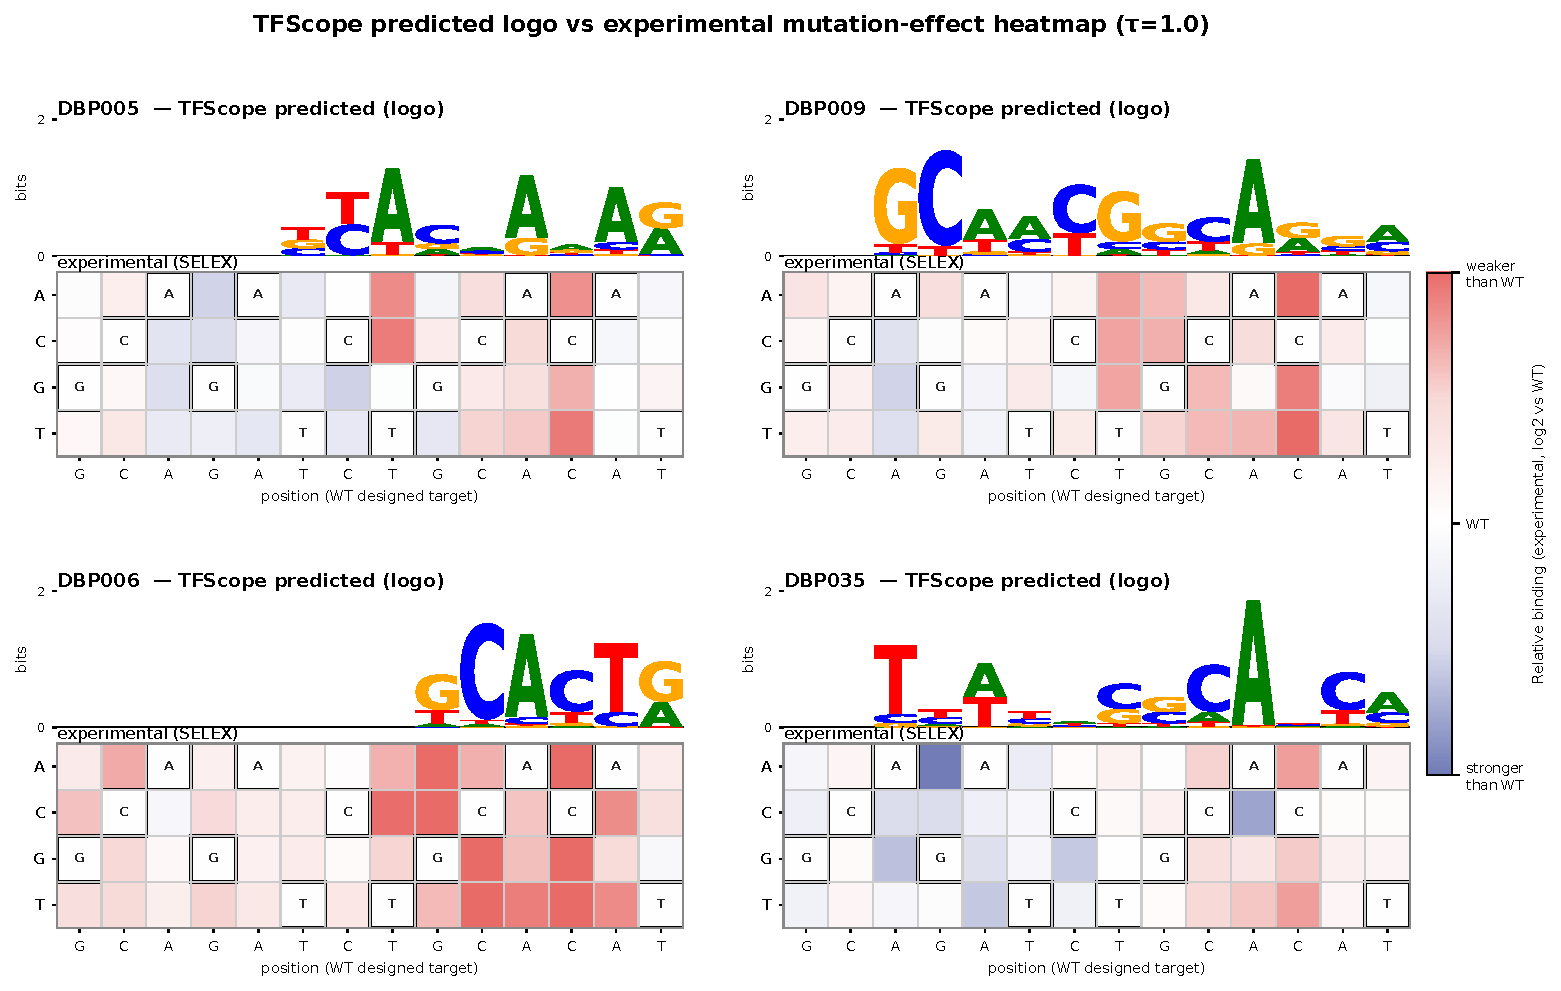
\includegraphics[width=\linewidth]{figures/dbp_tfscope_heatmap.pdf}
  \caption{\textbf{Sequence-only specificity prediction for de novo designed
    DNA-binding proteins.} For each designed protein (DBP5, DBP9, DBP6, DBP35; all
    engineered against 5$'$-GCAGATCTGCACATC-3$'$~\cite{Glasscock2025}), the
    TFScope-predicted position weight matrix (logo, top) is shown above the experimental
    single-base-pair mutation-effect heatmap (bottom; yeast-display relative binding,
    $\log_2$ versus the wild-type designed base; red, a substitution that weakens
    binding, \ie\ a specificity-determining position; blue, stronger than wild type; the
    wild-type base is boxed). From sequence alone TFScope recovers the central CAC core,
    most confidently for DBP6, where the predicted high-information CAC coincides with
    the experimentally specificity-determining columns; recovery is partial but
    consistent for DBP5/9/35.}
  \label{fig:designed}
\end{figure}

% ─────────────────────────────────────────────────────────────────────────────
\section*{Discussion}

TFScope shows that the binding-specificity information latent in a protein language
model, marshaled by architectural components for DBD pooling, family conditioning,
contact-aware attention, and homology retrieval, is sufficient to match or exceed
the structure-based state of the art for PWM prediction — without any structural
input. Five conclusions follow.

First, sequence alone is enough to reach the structural frontier. With retrieval
disabled TFScope already ties DeepPBS (mean $r$ 0.749 vs.\ 0.750) and exceeds it on
top-1 accuracy and Matthews correlation; with retrieval it leads on 8 of 11 metrics.
Because TFScope requires only the amino-acid sequence, it can be applied to all
\ts1,600 human TFs and to orthologues, paralogues, and disease variants across the
eukaryotic proteome at negligible cost — precisely the regime where docked complexes
are unavailable. Validation against the independent Codebook experimental
motifs~\cite{Codebook2024} confirms that this reach is real: on held-out,
sequence-distant factors the model recovers usable specificities for a meaningful
fraction of the dark proteome, with the zinc-finger class marking the current
ceiling.

Second, registration is the dominant remaining error. Both TFScope and DeepPBS shed
\ts0.43 in mean $r$ when motif placement is no longer granted by an oracle. Improving
where a motif is placed, rather than which bases it contains, is therefore the
highest-value next step, and motivates an explicit placement or gating head.

Third, retrieval is a learned homology-transfer operator, not a crutch. Its margin is
real but bounded, and it rests on a sequence encoder that is independently
competitive; rigorous leave-gene-out indexing is essential to measuring it honestly.

Fourth, in-distribution accuracy systematically overstates transfer. Leave-family-out
analysis reveals a \ts0.48 sequence-only transfer floor and shows that the
best-performing families in-distribution (bZIP, Homeodomain) owe much of their
accuracy to memorized family grammars. Closing the gap between this floor and the
in-distribution ceiling is the central open problem, and motivates anti-collapse
contrastive objectives~\cite{Bhatt2024} and large-scale protein--DNA pretraining.

Fifth, long C2H2 zinc-finger arrays are the frontier. Their per-finger recognition
codes violate the one-family-one-consensus assumption behind the family-conditioned
prior, producing the widest accuracy spread of any class. Consistent with this, the
mixture-of-experts decoder allocates its largest dedicated expert block to this
family, yet single shared experts cannot capture per-finger codes that differ from
one array to the next; a finger-resolved architecture that composes specificity from
individual fingers is the natural remedy.

TFScope has clear limitations. It predicts first-order PWMs and does not model
higher-order dependencies, cooperative or heterodimeric binding, or cofactor and
chromatin context; its attention localizes causal residues but its output is not yet
mutation-sensitive; and very long multi-domain proteins exceed its context window.
Each of these defines a concrete direction. Even so, by decoupling specificity
prediction from structure determination, TFScope makes proteome-scale, hypothesis-
generating annotation of TF binding preferences practical, and provides an
interpretable substrate on which these extensions can be built.

% ─────────────────────────────────────────────────────────────────────────────
\section*{Methods}

\subsection*{Data and preprocessing}
Training data were assembled from the DeepPBS dataset~\cite{Mitra2024} (520
TF--DNA crystal structures with validated PWMs) augmented with
CIS-BP~\cite{Weirauch2014}, RCADE, and MEME-derived entries, yielding 4,247 unique
TF records. Each record provides the amino-acid sequence, annotated DBD boundaries,
a family label among ten classes (bZIP, Homeodomain, Nuclear\_Receptor, Forkhead,
bHLH, C2H2\_short/medium/long, ETS, Other), and a $4\times L$ PWM ($L\leq20$). Each
PWM was trimmed to its IC\,$\geq$\,0.25 core; strand was canonicalized by selecting
the orientation whose 5$'$ end is more GC-rich, matching the
CIS-BP/JASPAR~\cite{CastroMondragon2022} convention.

\subsection*{Model architecture}
The encoder is ESM-2 (esm2\_t33\_650M\_UR50D)~\cite{Lin2023}, frozen, with LoRA
adapters (rank 16, $\alpha$ 32) on the last six layers and a learned 16-dimensional
DBD indicator embedding added within the DBD. Two gated attention-pooling modules
(global and DBD streams) yield 1280-dimensional vectors that are concatenated and
projected by Linear(2560$\to$512)$+$LayerNorm$+$GELU$+$Dropout(0.1). The decoder is
a DeepSeek-MoE-style block~\cite{Dai2024} (12 routed $+$ 1 shared experts, top-2
routing, load-balance weight 0.01) conditioned on 2304-dimensional semantic family
embeddings. The contact-aware PWM head freezes the legacy cross-attention as a prior
and adds a residual branch
$z = z_{\mathrm{prior}} + \lambda\,\Delta z_{\mathrm{contact}}$, where the contact
branch uses cosine cross-attention, LayerNorm on keys/values, amino-acid-identity
values, and row-diversity and hub penalties to prevent attention collapse;
$\lambda$ is a learned scalar and only the 0.55\,M contact-branch parameters are
trained. A two-layer MLP position gate emits per-column activation probabilities,
and a convolutional regression head emits $(4\times20)$ logits passed through a
per-column softmax. The retrieval branch injects $K$=3 nearest neighbors (cosine
similarity of the ESM-2 DBD representation) through a cross-attention layer before
the decoder; the LGO index excludes any neighbor sharing the query's gene symbol.

\subsection*{Training}
Models were optimized with AdamW (learning rate $6\times10^{-4}$, weight decay 0.01,
$\beta_1$=0.9, $\beta_2$=0.999), 500-step warmup and cosine decay, batch size 128,
and maximum sequence length 1024. The composite loss combined IC-weighted MSE and
per-column cross-entropy for PWM reconstruction, binary cross-entropy on the
IC\,$\geq$\,0.25 indicator for gate supervision, the MoE load-balance term, and an
optional in-batch contrastive PWM loss (weight 0.3, temperature 0.1). Training ran
on NVIDIA A100 (80\,GB) GPUs with early stopping on validation oracle $r$. The
DeepPBS-split model trained only the contact branch on 520 TFs; the cluster40 model
trained the full architecture from scratch on 2,983 TFs (best epoch 125); the ten
leave-family-out models each trained up to 200 epochs with one family held out,
using that family's correct semantic embedding so the prior carries no label
information.

\subsection*{Benchmarks}
\textit{cluster40} was built with CD-HIT~\cite{LiGodzik2006} at 40\% identity over
1,320 proteins (389 clusters), family-stratified 2,983/625/639. \textit{Leave-family-out}
splits held out each of the ten families in turn, drawing validation from the
remaining families by 40\%-identity clustering. DeepPBS predictions were read from
the published blind-benchmark output ($n$=130) and passed through the identical
trimmed-core oracle aligner; for the deployable protocol, both methods' outputs were
canonicalized identically.

\subsection*{Evaluation}
The primary metric is per-TF oracle Pearson $r$: gate-active predicted columns are
aligned to the IC\,$\geq$\,0.25 target core (offset $\pm$10, reverse-complement) and
$r$ is averaged column-wise. The supporting panel adds IC-weighted $r$, MAE, RMSE,
cross-entropy, KL divergence, top-1 (argmax) accuracy, macro AUC, macro F1, and MCC.
For the deployable protocol, prediction and target are canonicalized independently
and scored without alignment.

\subsection*{Attention analysis}
KLF4 and MyoD DBD sequences were run with retrieval disabled through the model with
and without the contact branch. Row-constancy is the mean off-diagonal correlation
among attention rows; entropy is the Shannon entropy of the column-averaged
attention distribution; residue mass is the summed attention at the annotated
recognition residue. Output mutation sensitivity was assessed by comparing
wild-type and single-point-mutant output PWMs.

\subsection*{Mutation switch score}
Wild-type and L122R MyoD basic-helix--loop--helix DBD sequences were run through the
model (retrieval disabled). For a predicted PWM $P$ and an E-box $s$, the score $S(s)$
is the maximum log-odds of $s$ against a uniform background ($\log_2 P/0.25$), taken
over all offsets and both strands. The directional switch score is
$\Delta_{\text{switch}} = [S_{\text{mut}}(\text{CACGTG}) - S_{\text{mut}}(\text{CACCTG})]
- [S_{\text{WT}}(\text{CACGTG}) - S_{\text{WT}}(\text{CACCTG})]$; positive values indicate
a predicted shift toward the MYC-like CACGTG. A difference-in-differences is used in
place of a consensus comparison because the single most-probable base is unstable to
small changes in the predicted distribution.

\subsection*{Designed-protein evaluation}
The four de novo designed proteins (DBP5, DBP6, DBP9, DBP35) and the experimental
single-base-pair binding data were taken from the design study~\cite{Glasscock2025}.
Each designed sequence was scored with the combined model (retrieval disabled), and the
predicted core was aligned to the 14-bp designed target. Experimental relative binding
per substituted base was computed as $\log_2(v/v_{\text{WT}})$, where $v$ is the
normalized median PE/FITC signal (lower signal indicates stronger binding); the
wild-type base is the reference. TFScope's predicted preference, $\log_2(P_{\text{WT}}/P_b)$,
was compared with the experimental landscape by per-position argmax agreement and
column-wise Pearson correlation over the aligned core.

% ─────────────────────────────────────────────────────────────────────────────
\section*{Data availability}
DeepPBS benchmark data are available from the original publication~\cite{Mitra2024}.
CIS-BP~\cite{Weirauch2014} and JASPAR~\cite{CastroMondragon2022} data are available
at \url{http://cisbp.ccbr.utoronto.ca/} and \url{http://jaspar.genereg.net/}. The
augmented training dataset and all splits will be deposited to Zenodo upon
acceptance.

\section*{Code availability}
TFScope source code and trained checkpoints will be released publicly upon
acceptance.

\section*{Funding}
[Funding sources to be completed.]

\section*{Acknowledgements}
[To be completed.]

\section*{Author contributions}
L.H. conceived the study, designed and implemented TFScope, performed all
experiments, and wrote the manuscript. [Co-author contributions TBD.]

\section*{Competing interests}
The authors declare no competing interests.

% ─────────────────────────────────────────────────────────────────────────────
\bibliographystyle{unsrtnat}
\bibliography{TFScope_refs}

% ─────────────────────────────────────────────────────────────────────────────
\clearpage
\setcounter{figure}{0}

\begin{figure}[p]
  \centering
  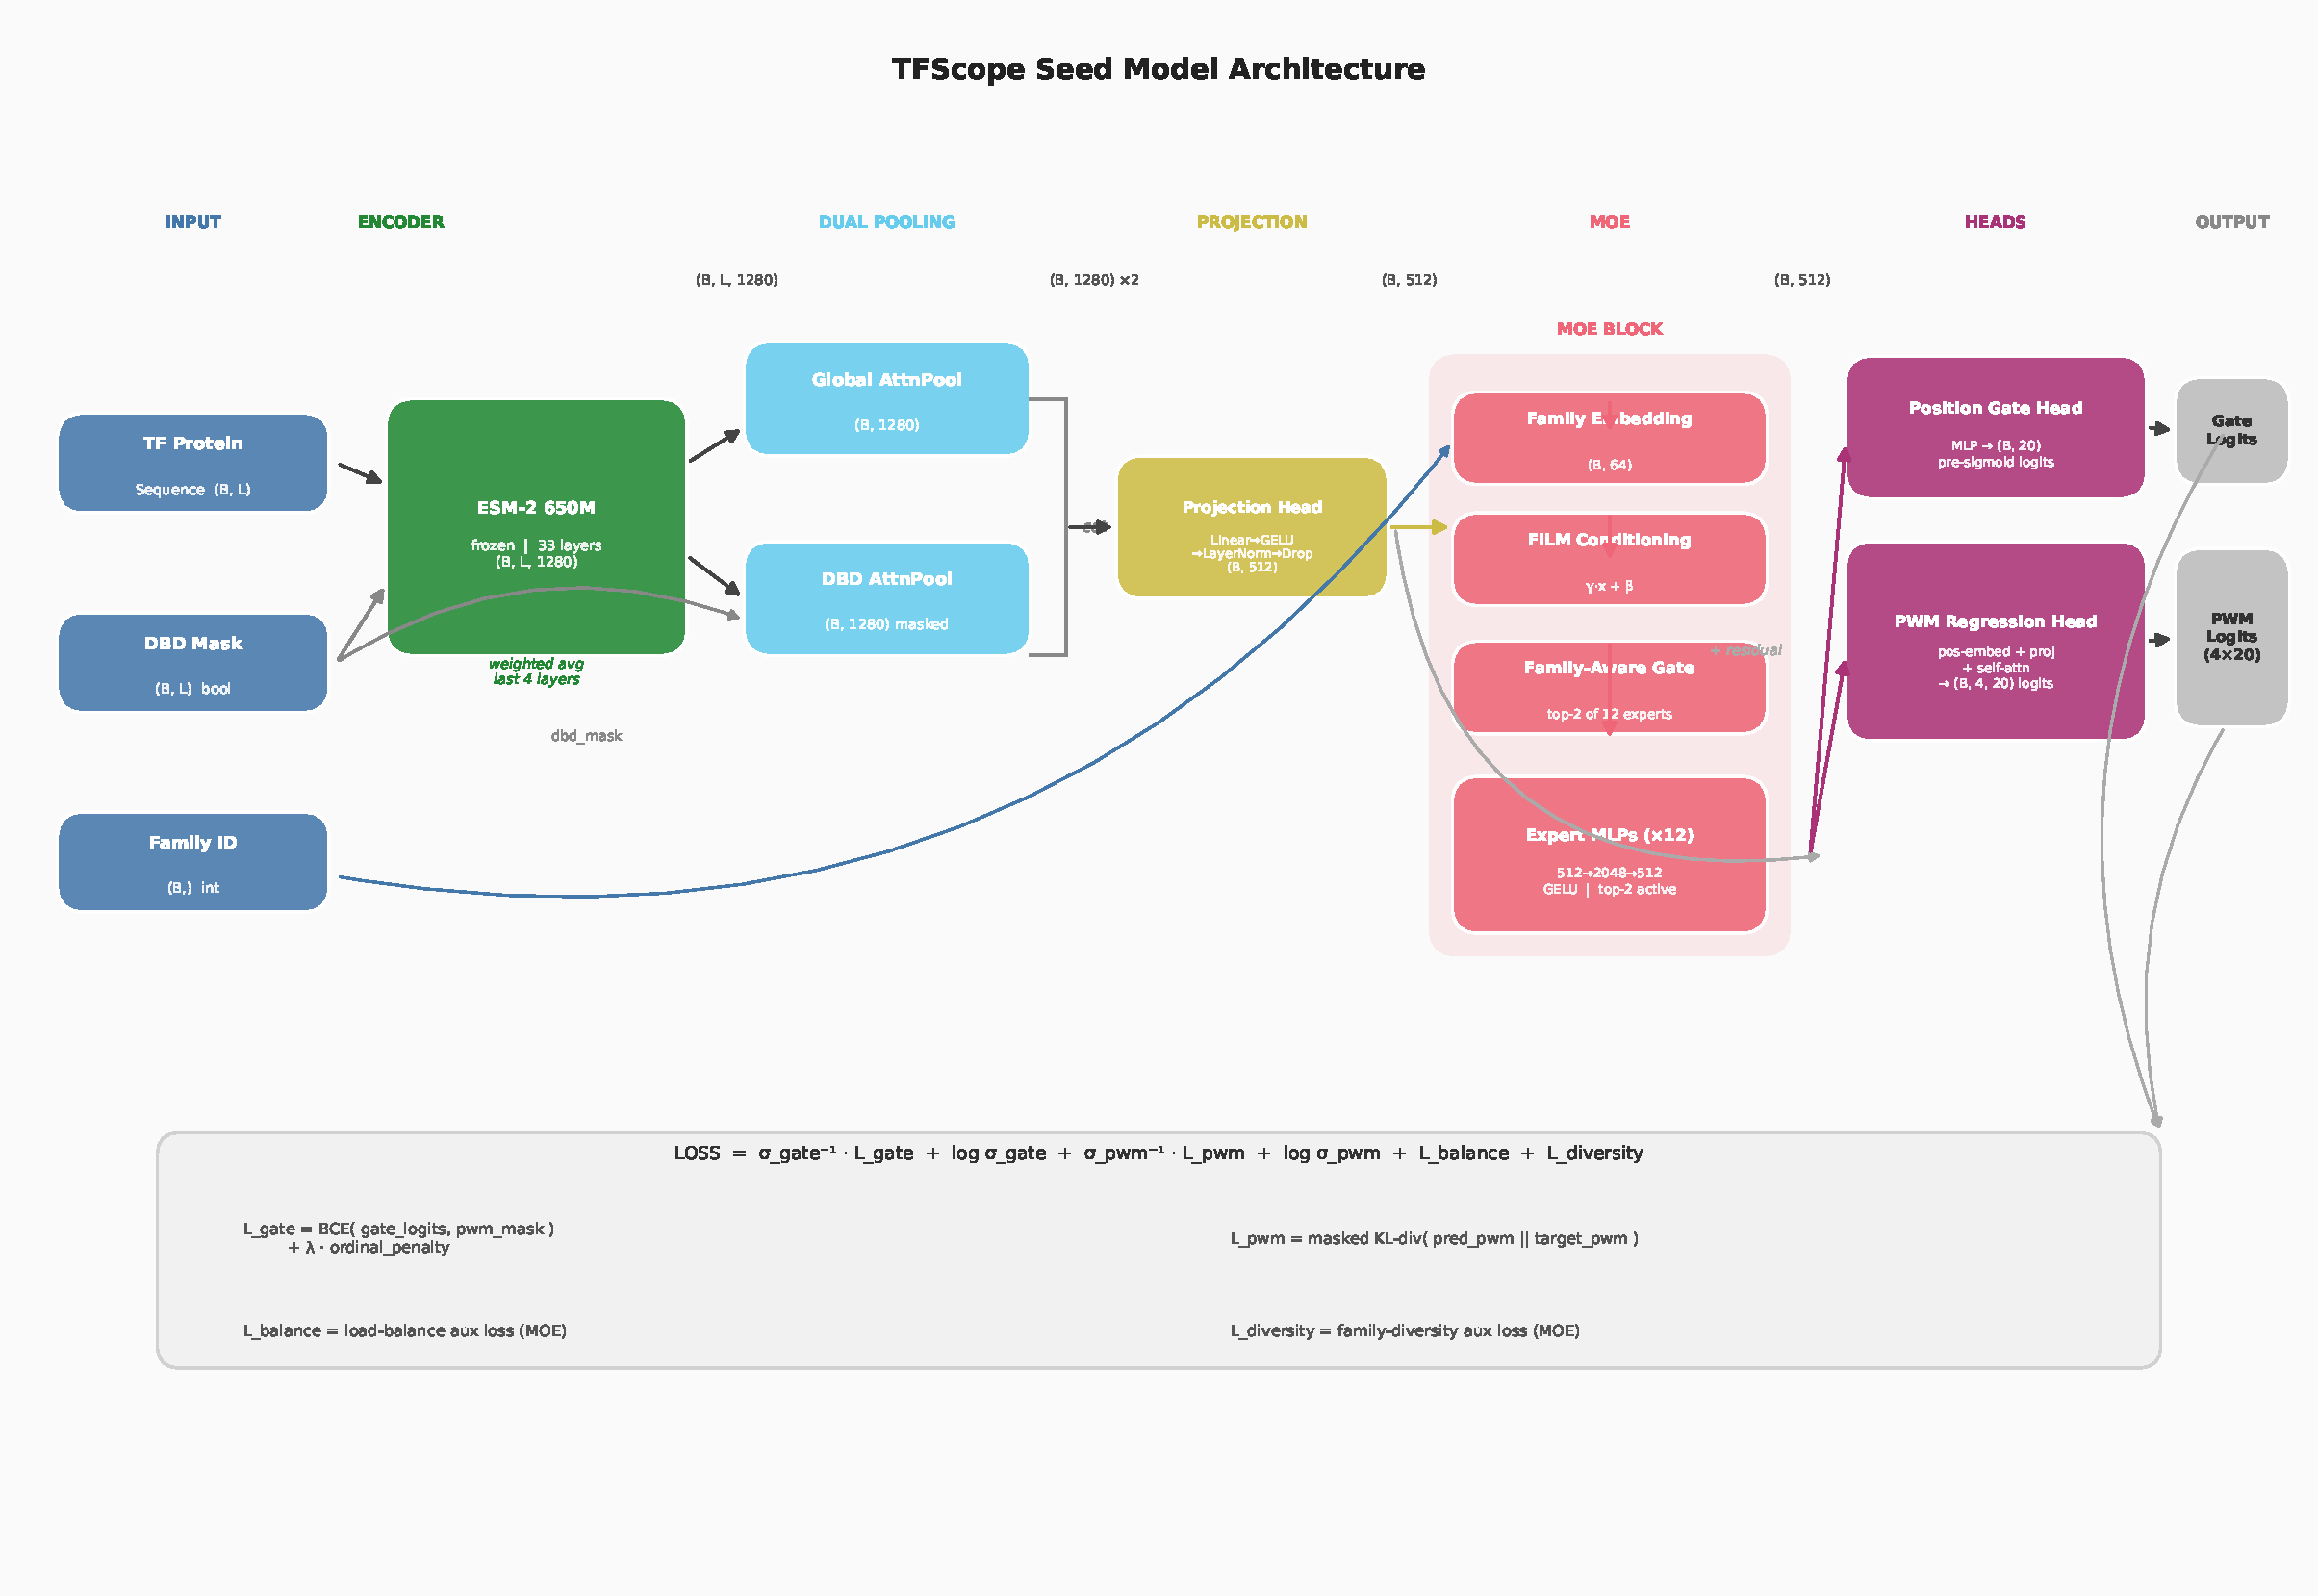
\includegraphics[width=\linewidth]{figures/tfscope_architecture.pdf}
  \caption{\textbf{The TFScope framework.}
    A TF amino-acid sequence passes through (i) a frozen ESM-2 encoder with LoRA
    adapters and a DBD indicator embedding; (ii) dual-stream gated pooling over the
    full sequence and the DBD; (iii) a family-conditioned mixture-of-experts decoder
    (12 routed $+$ 1 shared expert, top-2 routing) driven by semantic family
    embeddings; (iv) a contact-aware cross-attention head that augments a frozen
    prior with a $\lambda$-weighted residual branch; and (v) a position gate and PWM
    regression head. An optional leave-gene-out retrieval branch injects $K$=3
    nearest-neighbor PWMs before the decoder. Only \ts0.55\,M parameters
    (contact branch) are trained on the DeepPBS split; the encoder and prior remain
    frozen.}
  \label{fig:architecture}
\end{figure}

\begin{figure}[p]
  \centering
  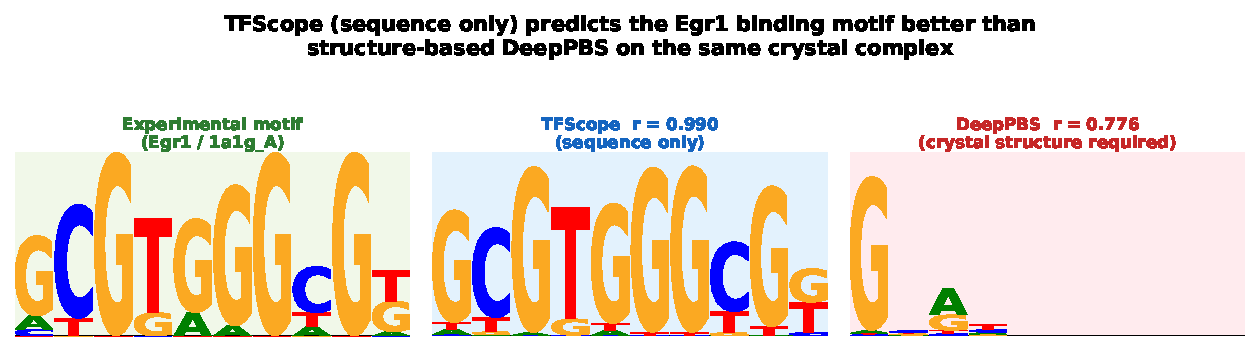
\includegraphics[width=0.86\linewidth]{figures/cs1_egr1_headtohead.pdf}
  \caption{\textbf{Sequence beats structure on the zinc-finger code (Egr1).}
    Sequence logos for Egr1/Zif268 (PDB 1a1g, chain A): the experimental motif
    (JASPAR MA0162.1; top), the TFScope prediction from sequence alone
    (oracle $r$=0.990; middle), and the DeepPBS prediction from the crystal complex
    (oracle $r$=0.776; bottom). Egr1 reads its 10-bp GC-rich site finger-by-finger
    via recognition-helix residues~\cite{Pavletich1991}; TFScope reconstructs all
    three GCG subsites, whereas the structure-based prediction is nearly flat.}
  \label{fig:egr1}
\end{figure}

\begin{figure}[p]
  \centering
  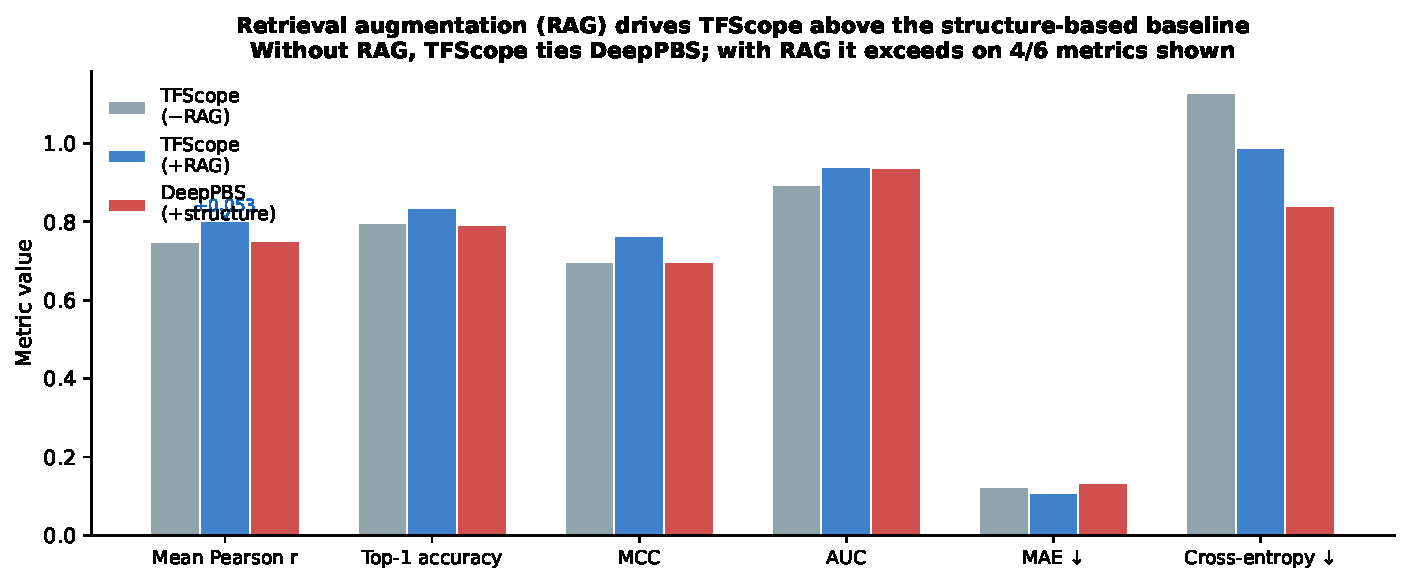
\includegraphics[width=\linewidth]{figures/cs_rag_ablation.pdf}
  \caption{\textbf{The sequence encoder alone matches DeepPBS; retrieval extends the
    lead.}
    Six motif-level metrics on the 130-TF DeepPBS blind split for TFScope without
    retrieval ($-$RAG), TFScope with retrieval, and DeepPBS. Without retrieval,
    TFScope ties DeepPBS on mean $r$ (0.749 vs.\ 0.750) and already exceeds it on
    top-1 accuracy and MCC; retrieval raises mean $r$ to 0.802. DeepPBS retains an
    advantage only on calibration (cross-entropy, KL).}
  \label{fig:rag}
\end{figure}

\begin{figure}[p]
  \centering
  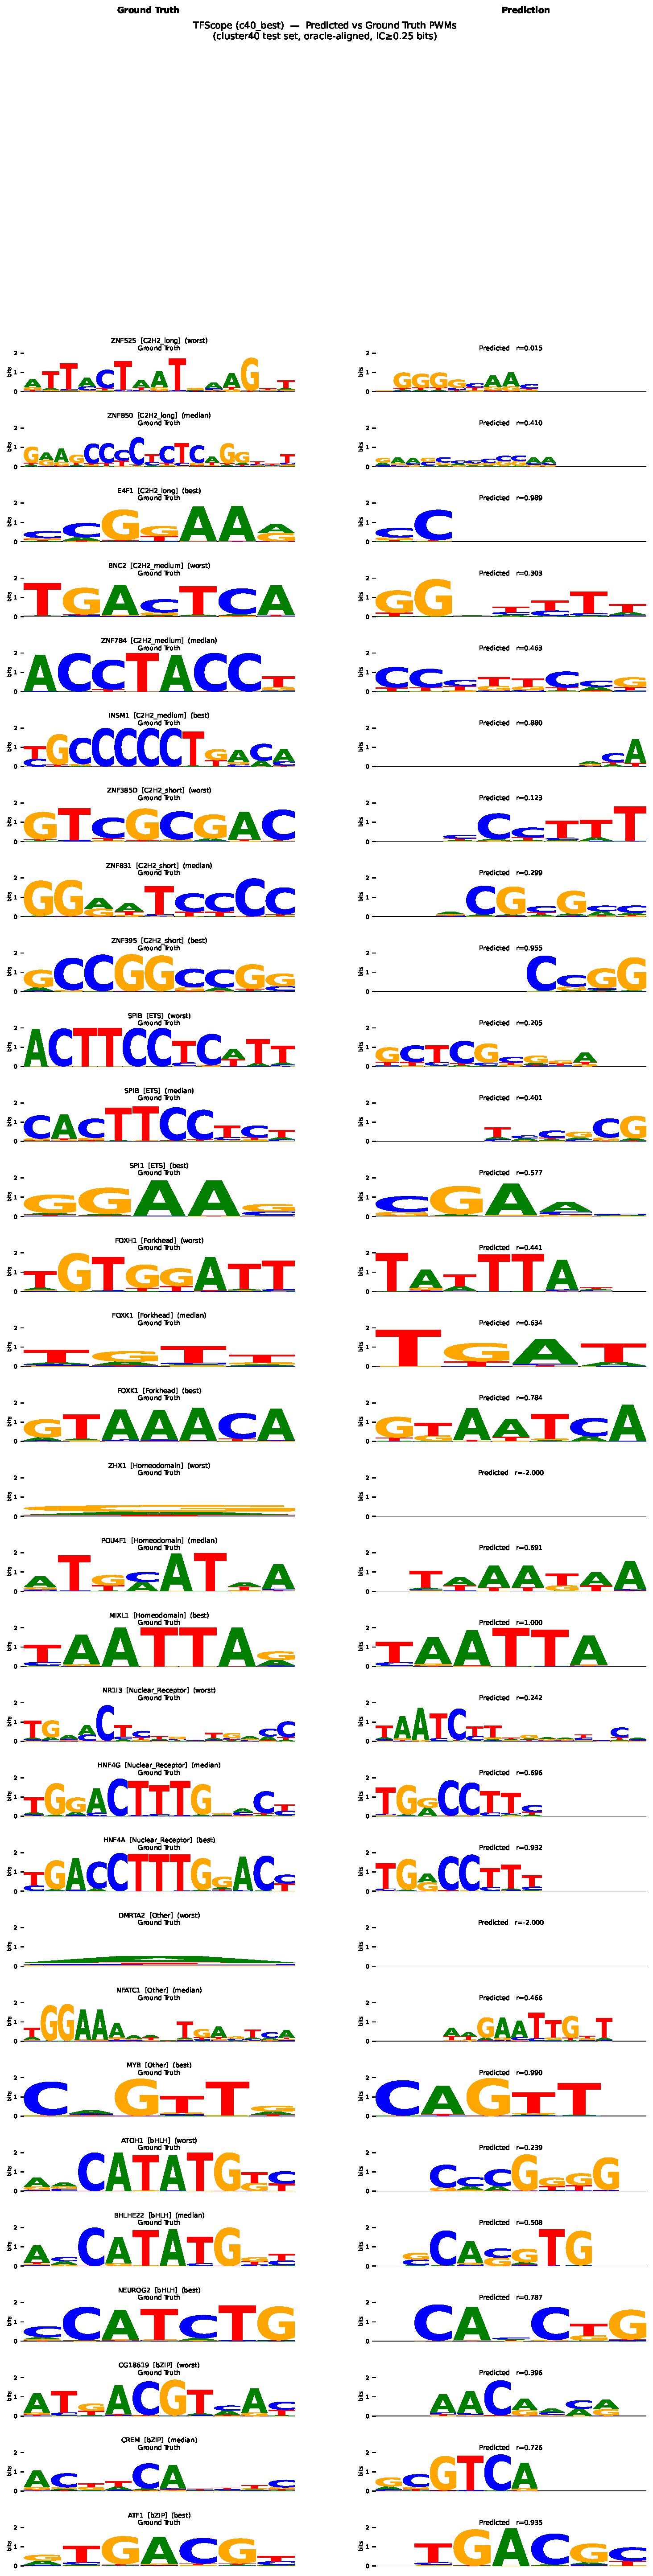
\includegraphics[width=\linewidth]{figures/pred_vs_gt_cluster40.pdf}
  \caption{\textbf{Out-of-distribution generalization (cluster40).}
    Ground-truth (left) and TFScope-predicted (right) logos for representative TFs
    from the 639-TF cluster40 held-out set (mean oracle $r$=0.535); no test TF
    shares $>$40\% identity with any training TF. Oracle $r$ is annotated per pair.}
  \label{fig:ood}
\end{figure}

\begin{figure}[p]
  \centering
  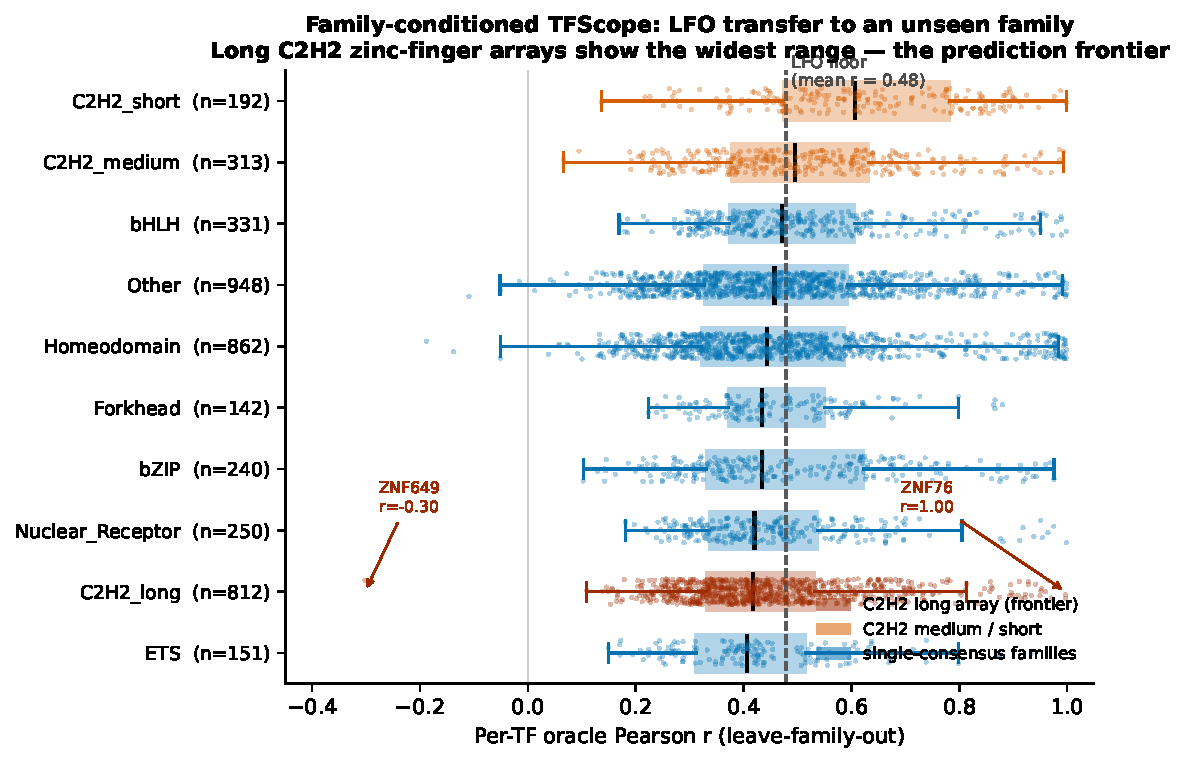
\includegraphics[width=\linewidth]{figures/cs3_family_frontier.pdf}
  \caption{\textbf{A sequence-only transfer floor and the C2H2 frontier
    (leave-family-out).}
    Per-TF oracle $r$ under leave-family-out for all ten families (4,241 TFs),
    ordered by median. The dashed line marks the macro-average transfer floor
    ($r$=0.479). The broad in-distribution spread compresses to a tight transfer
    band; long C2H2 arrays (darker) show the lowest mean and the widest spread,
    marking them as the prediction frontier.}
  \label{fig:lfo}
\end{figure}

\begin{figure}[p]
  \centering
  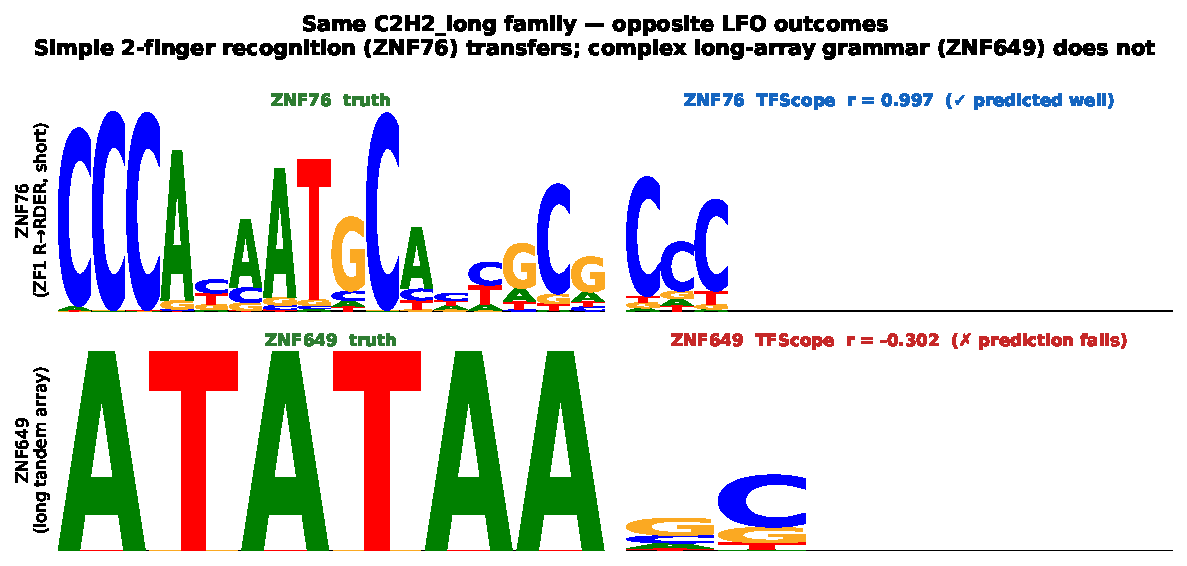
\includegraphics[width=0.86\linewidth]{figures/cs3_znf_examples.pdf}
  \caption{\textbf{Per-finger code complexity decides outcomes in long C2H2 arrays.}
    Experimental (top) and TFScope-predicted (bottom) logos for the best- and
    worst-transferring C2H2\_long TFs under leave-family-out. ZNF76, dominated by a
    short repetitive finger grammar, is reconstructed almost perfectly
    (oracle $r$=0.997); ZNF649, a long array with a complex per-finger code and an
    AT-rich target, collapses to near-random ($r$=$-$0.302). Both had their entire
    family held out.}
  \label{fig:znf}
\end{figure}

\begin{figure}[p]
  \centering
  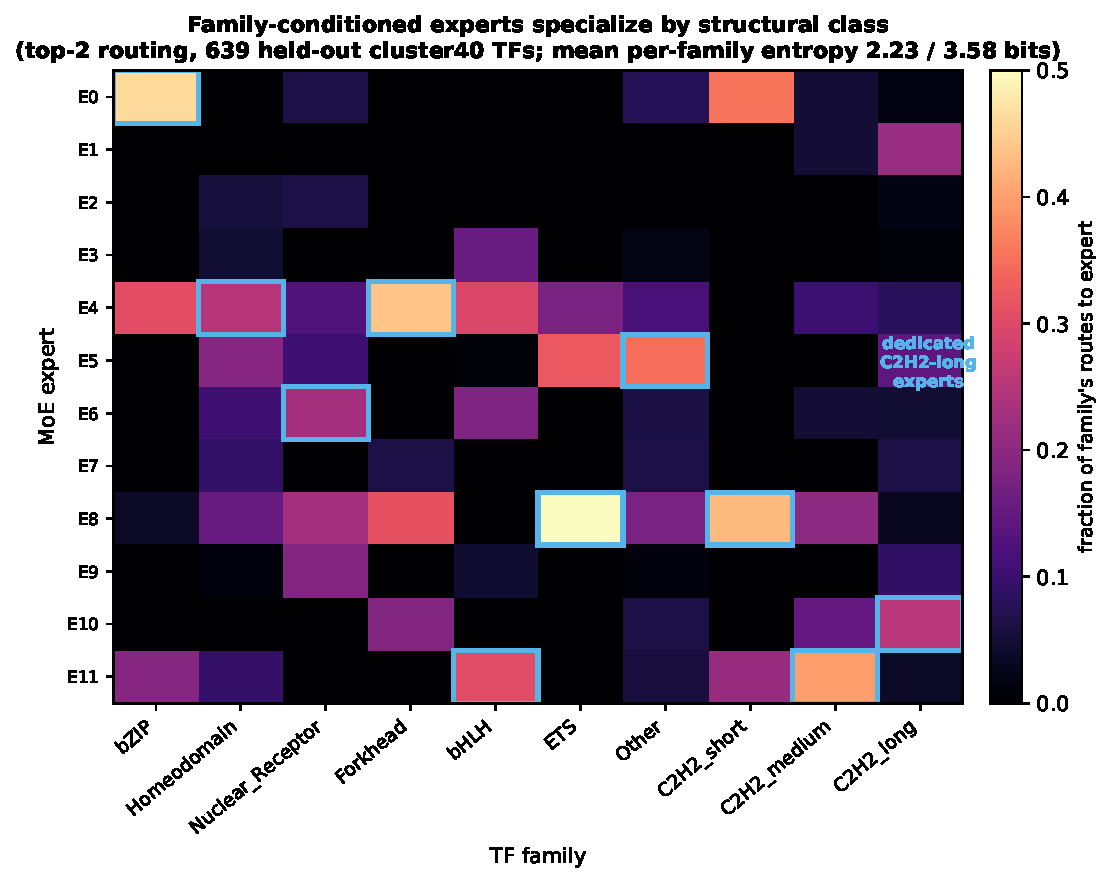
\includegraphics[width=0.82\linewidth]{figures/cs_moe_routing.pdf}
  \caption{\textbf{Family-conditioned experts specialize by structural class.}
    Column-normalized top-2 routing frequency of each TF family (columns) over the
    twelve routed experts (rows), measured on the 639 held-out cluster40 TFs. Cyan
    boxes mark each family's dominant expert. Routing is strongly family-structured
    (mean per-family entropy 2.23 of a possible 3.58 bits): one expert is a near-pure
    C2H2\_long specialist (98.7\%) and a cluster of three experts is C2H2\_long-dominated,
    giving the prediction-frontier family the largest dedicated capacity, while a
    separate expert specializes in Homeodomains. Compact single-consensus families
    share higher-usage generalist experts. Specialization measured on
    out-of-distribution TFs indicates it generalizes beyond training identities.}
  \label{fig:moe}
\end{figure}

\begin{figure}[p]
  \centering
  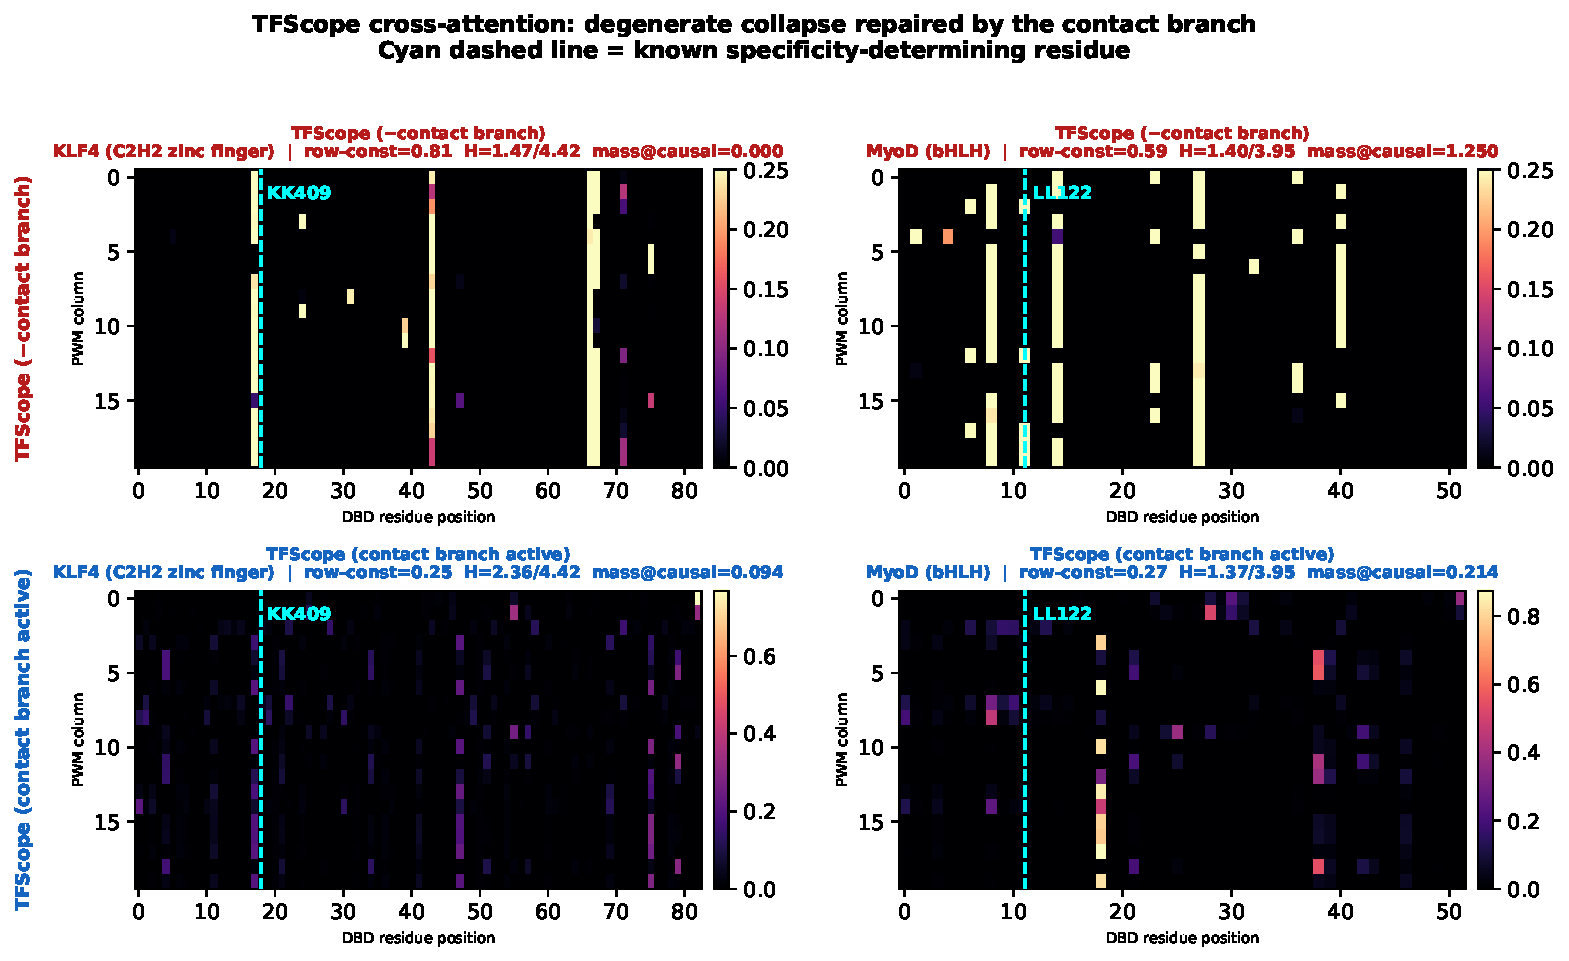
\includegraphics[width=\linewidth]{figures/cs2_klf4_attention_repair.pdf}
  \caption{\textbf{Cross-attention concentrates on base-contacting residues.}
    Attention from each PWM column ($y$) to each DBD residue ($x$) for KLF4 (C2H2)
    and MyoD (bHLH), without (top) and with (bottom) the contact-aware branch. The
    cyan line marks the experimentally identified recognition residue (KLF4 K409;
    MyoD L122). The contact branch breaks the degenerate rank-1 pattern (KLF4
    row-constancy 0.81$\to$0.25) and directs attention onto the recognition residue,
    recovering the correct recognition chemistry without structural supervision.}
  \label{fig:attn}
\end{figure}

\begin{figure}[p]
  \centering
  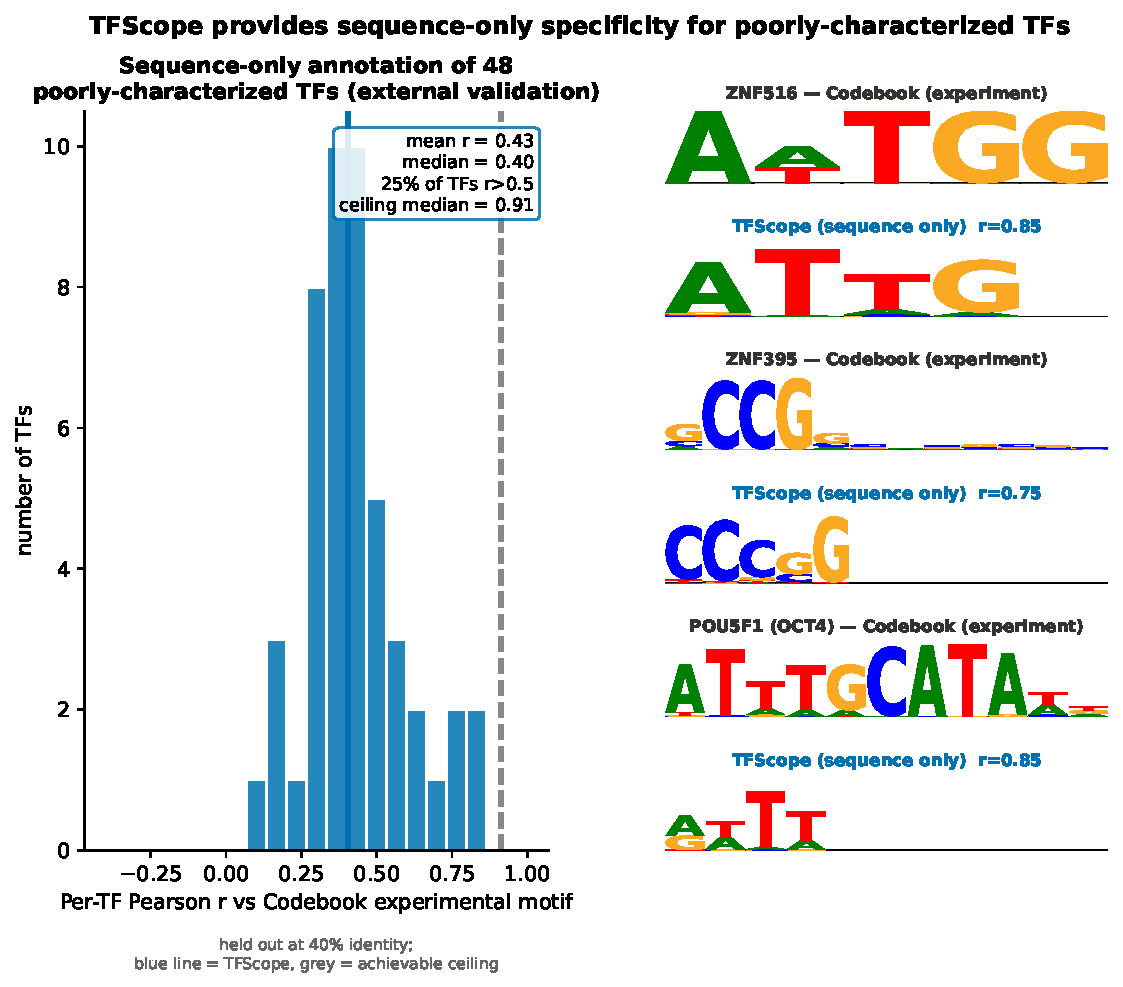
\includegraphics[width=\linewidth]{figures/cs_codebook_external.pdf}
  \caption{\textbf{Sequence-only annotation of poorly-characterized TFs, validated
    against external Codebook motifs.}
    \textbf{Left}, distribution of per-TF Pearson $r$ between TFScope's sequence-only
    prediction and the independent Codebook expert-curated experimental
    motif~\cite{Codebook2024}, for the 48 Codebook TFs in our cluster40 held-out
    partition (held out at 40\% identity; never seen by the model). Blue line, TFScope
    median; grey dashed line, the database-concordance ceiling (our own database
    targets vs.\ Codebook), which bounds achievable accuracy. \textbf{Right}, example
    motifs (Codebook experimental, top; TFScope prediction, bottom) for two dark
    zinc-finger factors (ZNF516, ZNF395) and the pluripotency factor POU5F1/OCT4, all
    reconstructed from protein sequence alone. The set is zinc-finger-dominated,
    placing it at the model's honest frontier; nonetheless a substantial fraction of
    these otherwise-uncharacterized factors receive usable specificity annotations.}
  \label{fig:codebook}
\end{figure}

% ─────────────────────────────────────────────────────────────────────────────
\clearpage

\begin{table}[p]
\centering
\caption{\textbf{Motif-level accuracy on the DeepPBS 130-TF blind split.}
  Oracle-aligned protocol (IC\,$\geq$\,0.25 core, offset$\pm$10 and
  reverse-complement alignment), $n$=116 TFs covered by all methods. Bold marks
  the better of TFScope vs.\ DeepPBS. For CE and KL, lower is better. The final two
  rows give the deployable canonical-fixed mean $r$ (no alignment oracle), where the
  two methods tie.}
\label{tab:bench1}
\smallskip
\renewcommand{\arraystretch}{1.2}
\begin{tabular}{@{}lccc@{}}
\toprule
\textbf{Metric} & \textbf{TFScope ($-$contact)} & \textbf{TFScope} & \textbf{DeepPBS} \\
\midrule
Mean Pearson $r$        & 0.701 & \textbf{0.802} & 0.750 \\
Median Pearson $r$      & 0.723 & \textbf{0.831} & 0.759 \\
Top-1 accuracy          & 0.753 & \textbf{0.836} & 0.793 \\
MCC                     & 0.615 & \textbf{0.765} & 0.698 \\
F1 score                & 0.646 & \textbf{0.765} & 0.724 \\
AUC                     & 0.879 & \textbf{0.939} & 0.937 \\
IC-weighted $r$         & 0.954 & \textbf{0.972} & 0.968 \\
MAE                     & 0.141 & \textbf{0.108} & 0.133 \\
RMSE                    & 0.242 & \textbf{0.184} & 0.204 \\
Cross-entropy (CE)      & 1.140 & 0.988          & \textbf{0.840} \\
KL divergence           & 0.666 & 0.517          & \textbf{0.358} \\
\midrule
\multicolumn{4}{@{}l}{\textit{Deployable (canonical-fixed, no alignment oracle)}}\\
Mean Pearson $r$        & --- & 0.420 & 0.419 \\
\bottomrule
\end{tabular}
\end{table}

\begin{table}[p]
\centering
\caption{\textbf{Retrieval ablation on the DeepPBS blind split.}
  With retrieval disabled, the TFScope sequence encoder alone already matches
  DeepPBS on mean $r$ and exceeds it on top-1 accuracy and MCC; retrieval extends
  the margin across all base-composition metrics.}
\label{tab:rag}
\smallskip
\renewcommand{\arraystretch}{1.2}
\begin{tabular}{@{}lccc@{}}
\toprule
\textbf{Metric} & \textbf{TFScope $-$RAG} & \textbf{TFScope $+$RAG} & \textbf{DeepPBS} \\
\midrule
Mean Pearson $r$ & 0.749 & \textbf{0.802} & 0.750 \\
Top-1 accuracy   & 0.797 & \textbf{0.836} & 0.793 \\
MCC              & 0.699 & \textbf{0.765} & 0.698 \\
F1 score         & 0.696 & \textbf{0.765} & 0.724 \\
MAE              & 0.124 & \textbf{0.108} & 0.133 \\
Cross-entropy    & 1.129 & 0.988          & \textbf{0.840} \\
\bottomrule
\end{tabular}
\end{table}

\begin{table}[p]
\centering
\caption{\textbf{Out-of-distribution accuracy on cluster40.}
  639-TF held-out set; no test TF within 40\% identity of any training TF. Model
  trained from scratch on 2,983 cluster40 training TFs.}
\label{tab:ood}
\smallskip
\renewcommand{\arraystretch}{1.2}
\begin{tabular}{@{}lc@{}}
\toprule
\textbf{Metric} & \textbf{TFScope (cluster40)} \\
\midrule
Mean oracle $r$   & 0.535 \\
Median oracle $r$ & 0.505 \\
IC-weighted $r$   & 0.553 \\
Top-1 accuracy    & 0.630 \\
AUC               & 0.797 \\
F1 score          & 0.603 \\
MCC               & 0.472 \\
MAE               & 0.198 \\
\bottomrule
\end{tabular}
\end{table}

\begin{table}[p]
\centering
\caption{\textbf{Leave-family-out transfer by family.}
  Each model was trained with the named family entirely held out and evaluated on
  that family; values are reproduced from per-TF scores. Families are ordered by
  mean transfer $r$. The $\Delta$ column gives the change from the same family's
  cluster40 in-distribution score where available, capturing family memorization;
  large negative values indicate accuracy that does not transfer.}
\label{tab:lfo}
\smallskip
\renewcommand{\arraystretch}{1.2}
\begin{tabular}{@{}lcccc@{}}
\toprule
\textbf{Family} & \textbf{$n$} & \textbf{Mean $r$} & \textbf{Median $r$} & \textbf{$\Delta$ in-dist} \\
\midrule
ETS               & 151 & 0.424 & 0.407 & --- \\
C2H2\_long        & 812 & 0.447 & 0.417 & $+$0.017 \\
Nuclear\_Receptor & 250 & 0.454 & 0.421 & --- \\
Forkhead          & 142 & 0.464 & 0.435 & --- \\
Other             & 948 & 0.473 & 0.457 & --- \\
Homeodomain       & 862 & 0.478 & 0.443 & $-$0.202 \\
bZIP              & 240 & 0.485 & 0.434 & $-$0.235 \\
bHLH              & 331 & 0.508 & 0.471 & $+$0.008 \\
C2H2\_medium      & 313 & 0.514 & 0.495 & $+$0.014 \\
C2H2\_short       & 192 & 0.613 & 0.606 & $+$0.223 \\
\midrule
\textbf{Macro avg} & \textbf{4241} & \textbf{0.479} & \textbf{0.447} & --- \\
\bottomrule
\end{tabular}
\end{table}

\end{document}
